\documentclass[tikz,border=10pt]{standalone}
\usepackage{tikz}
\usetikzlibrary{positioning}

\begin{document}

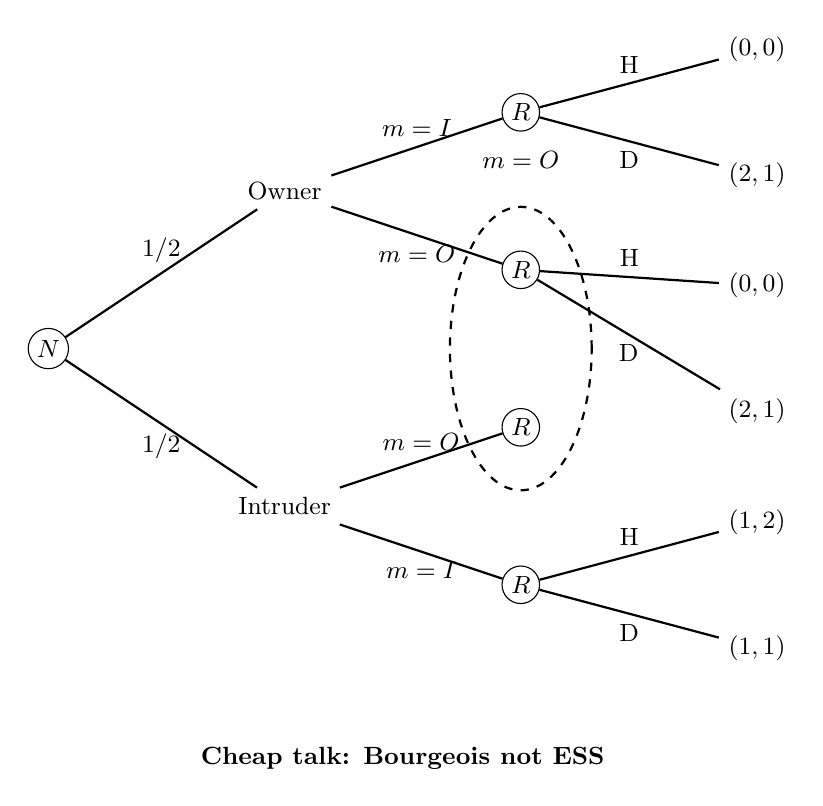
\begin{tikzpicture}[
    font=\small,
    decision/.style={circle,draw,inner sep=1.5pt},
    chance/.style={circle,draw,inner sep=1.5pt},
    line/.style={thick},
    infoset/.style={thick,dashed}
]

% Nature
\node[chance] (N) at (0,0) {$N$};

% Types
\node (O) at (3,2) {Owner};
\node (I) at (3,-2) {Intruder};

\draw[line] (N) -- node[above] {$1/2$} (O);
\draw[line] (N) -- node[below] {$1/2$} (I);

% Receiver nodes
\node[decision] (SO1) at (6,3) {$R$};   % Owner -> O
\node[decision] (SO2) at (6,1) {$R$};   % Owner -> I
\node[decision] (SI1) at (6,-1) {$R$};  % Intruder -> O
\node[decision] (SI2) at (6,-3) {$R$};  % Intruder -> I

% Messages (SWAPPED at Owner)
\draw[line] (O) -- node[above] {$m=I$} (SO1);
\draw[line] (O) -- node[below] {$m=O$} (SO2);

\draw[line] (I) -- node[above] {$m=O$} (SI1);
\draw[line] (I) -- node[below] {$m=I$} (SI2);

% Information set for m = O (CORRECT)
\draw[infoset] (6,0) ellipse (0.9 and 1.8);

\node at (6,2.4) {$m=O$};

% Payoffs
\node (S1) at (9,3.8) {$(0,0)$};
\node (S2) at (9,2.2) {$(2,1)$};
\node (S3) at (9,0.8) {$(0,0)$};
\node (S4) at (9,-0.8) {$(2,1)$};
\node (S5) at (9,-2.2) {$(1,2)$};
\node (S6) at (9,-3.8) {$(1,1)$};

\draw[line] (SO1) -- node[above] {H} (S1);
\draw[line] (SO1) -- node[below] {D} (S2);

\draw[line] (SO2) -- node[above] {H} (S3);
\draw[line] (SO2) -- node[below] {D} (S4);

\draw[line] (SI2) -- node[above] {H} (S5);
\draw[line] (SI2) -- node[below] {D} (S6);

\node at (4.5,-5.2) {\textbf{Cheap talk: Bourgeois not ESS}};

\end{tikzpicture}

\end{document}
